%*----------- SLIDE -------------------------------------------------------------
% \begin{frame}[t]{Introdução} 
    
%     \begin{tikzpicture}[thick , scale=1, every  node/.style={scale =0.75}]
%         \node[at=(current  page.center)]
%         {
%             % Created by tikzDevice version 0.12.3.1 on 2022-01-16 03:35:37
% !TEX encoding = UTF-8 Unicode
\begin{tikzpicture}[x=1pt,y=1pt]
\definecolor{fillColor}{RGB}{255,255,255}
\path[use as bounding box,fill=fillColor,fill opacity=0.00] (0,0) rectangle (252.94,252.94);
\begin{scope}
\path[clip] (  0.00,  0.00) rectangle (252.94,252.94);
\definecolor{drawColor}{RGB}{0,0,0}
\definecolor{fillColor}{RGB}{255,0,0}

\path[draw=drawColor,line width= 0.4pt,line join=round,line cap=round,fill=fillColor] ( 55.81, 62.61) rectangle ( 79.43, 93.97);
\definecolor{fillColor}{RGB}{255,77,0}

\path[draw=drawColor,line width= 0.4pt,line join=round,line cap=round,fill=fillColor] ( 84.15, 62.61) rectangle (107.77,203.75);
\definecolor{fillColor}{RGB}{255,153,0}

\path[draw=drawColor,line width= 0.4pt,line join=round,line cap=round,fill=fillColor] (112.49, 62.61) rectangle (136.11, 78.29);
\definecolor{fillColor}{RGB}{255,229,0}

\path[draw=drawColor,line width= 0.4pt,line join=round,line cap=round,fill=fillColor] (140.83, 62.61) rectangle (164.45,188.06);
\definecolor{fillColor}{RGB}{204,255,0}

\path[draw=drawColor,line width= 0.4pt,line join=round,line cap=round,fill=fillColor] (169.17, 62.61) rectangle (192.79, 78.29);
\definecolor{fillColor}{RGB}{128,255,0}

\path[draw=drawColor,line width= 0.4pt,line join=round,line cap=round,fill=fillColor] (197.52, 62.61) rectangle (221.13,125.34);
\end{scope}
\end{tikzpicture}

%         };
%     \end{tikzpicture}

%     \note[item]{Notes can help you to remember important information. Turn on the notes option.}
% \end{frame}

%-
%*----------- SLIDE -------------------------------------------------------------
% \begin{frame}[t]{Introdução}

%     \begin{figure}
%         \subfloat[1° Mês]
%         \centering
%         {
%         \begin{tikzpicture}
%             \begin{tikzpicture}[thick , scale=0.5, every  node/.style={scale =0.5}]
%                 \node[at=(current  page.center)]
%                 {
%                     % Created by tikzDevice version 0.12.3.1 on 2022-01-16 03:35:37
% !TEX encoding = UTF-8 Unicode
\begin{tikzpicture}[x=1pt,y=1pt]
\definecolor{fillColor}{RGB}{255,255,255}
\path[use as bounding box,fill=fillColor,fill opacity=0.00] (0,0) rectangle (252.94,252.94);
\begin{scope}
\path[clip] (  0.00,  0.00) rectangle (252.94,252.94);
\definecolor{drawColor}{RGB}{0,0,0}
\definecolor{fillColor}{RGB}{255,0,0}

\path[draw=drawColor,line width= 0.4pt,line join=round,line cap=round,fill=fillColor] ( 55.81, 62.61) rectangle ( 79.43, 93.97);
\definecolor{fillColor}{RGB}{255,77,0}

\path[draw=drawColor,line width= 0.4pt,line join=round,line cap=round,fill=fillColor] ( 84.15, 62.61) rectangle (107.77,203.75);
\definecolor{fillColor}{RGB}{255,153,0}

\path[draw=drawColor,line width= 0.4pt,line join=round,line cap=round,fill=fillColor] (112.49, 62.61) rectangle (136.11, 78.29);
\definecolor{fillColor}{RGB}{255,229,0}

\path[draw=drawColor,line width= 0.4pt,line join=round,line cap=round,fill=fillColor] (140.83, 62.61) rectangle (164.45,188.06);
\definecolor{fillColor}{RGB}{204,255,0}

\path[draw=drawColor,line width= 0.4pt,line join=round,line cap=round,fill=fillColor] (169.17, 62.61) rectangle (192.79, 78.29);
\definecolor{fillColor}{RGB}{128,255,0}

\path[draw=drawColor,line width= 0.4pt,line join=round,line cap=round,fill=fillColor] (197.52, 62.61) rectangle (221.13,125.34);
\end{scope}
\end{tikzpicture}

%                 };
%             \end{tikzpicture}
%         \end{tikzpicture}
%         }
%         \subfloat[2° Mês]
%         \centering
%         {
%         \begin{tikzpicture}
%             \begin{tikzpicture}[thick , scale=0.5, every  node/.style={scale =0.5}]
%                 \node[at=(current  page.center)]
%                 {
%                     % Created by tikzDevice version 0.12.3.1 on 2022-01-16 03:37:54
% !TEX encoding = UTF-8 Unicode
\begin{tikzpicture}[x=1pt,y=1pt]
\definecolor{fillColor}{RGB}{255,255,255}
\path[use as bounding box,fill=fillColor,fill opacity=0.00] (0,0) rectangle (252.94,252.94);
\begin{scope}
\path[clip] (  0.00,  0.00) rectangle (252.94,252.94);
\definecolor{drawColor}{RGB}{0,0,0}
\definecolor{fillColor}{RGB}{255,0,0}

\path[draw=drawColor,line width= 0.4pt,line join=round,line cap=round,fill=fillColor] ( 55.81, 62.61) rectangle ( 91.75, 93.97);
\definecolor{fillColor}{RGB}{255,77,0}

\path[draw=drawColor,line width= 0.4pt,line join=round,line cap=round,fill=fillColor] ( 98.94, 62.61) rectangle (134.88,203.75);
\definecolor{fillColor}{RGB}{255,153,0}

\path[draw=drawColor,line width= 0.4pt,line join=round,line cap=round,fill=fillColor] (142.07, 62.61) rectangle (178.01,203.75);
\definecolor{fillColor}{RGB}{255,229,0}

\path[draw=drawColor,line width= 0.4pt,line join=round,line cap=round,fill=fillColor] (185.19, 62.61) rectangle (221.13,141.02);
\end{scope}
\end{tikzpicture}

%                 };
%             \end{tikzpicture}
%         \end{tikzpicture}
%         }
%         \subfloat[3° Mês]
%         \centering
%         {
%         \begin{tikzpicture}
%             \begin{tikzpicture}[thick , scale=0.5, every  node/.style={scale =0.5}]
%                 \node[at=(current  page.center)]
%                 {
%                     % Created by tikzDevice version 0.12.3.1 on 2022-01-16 03:37:59
% !TEX encoding = UTF-8 Unicode
\begin{tikzpicture}[x=1pt,y=1pt]
\definecolor{fillColor}{RGB}{255,255,255}
\path[use as bounding box,fill=fillColor,fill opacity=0.00] (0,0) rectangle (252.94,252.94);
\begin{scope}
\path[clip] (  0.00,  0.00) rectangle (252.94,252.94);
\definecolor{drawColor}{RGB}{0,0,0}
\definecolor{fillColor}{RGB}{255,0,0}

\path[draw=drawColor,line width= 0.4pt,line join=round,line cap=round,fill=fillColor] ( 55.81, 62.61) rectangle (104.44, 79.22);
\definecolor{fillColor}{RGB}{255,77,0}

\path[draw=drawColor,line width= 0.4pt,line join=round,line cap=round,fill=fillColor] (114.16, 62.61) rectangle (162.78,203.75);
\definecolor{fillColor}{RGB}{255,153,0}

\path[draw=drawColor,line width= 0.4pt,line join=round,line cap=round,fill=fillColor] (172.51, 62.61) rectangle (221.13,112.42);
\end{scope}
\end{tikzpicture}

%                 };
%             \end{tikzpicture}
%         \end{tikzpicture}
%         }
%         \end{figure}

%     \note[item]{Notes can help you to remember important information. Turn on the notes option.}
% \end{frame}

%*----------- SLIDE -------------------------------------------------------------
% \begin{frame}[c]{Quantidade de paradas}
%     \centering
%     \begin{figure}
%         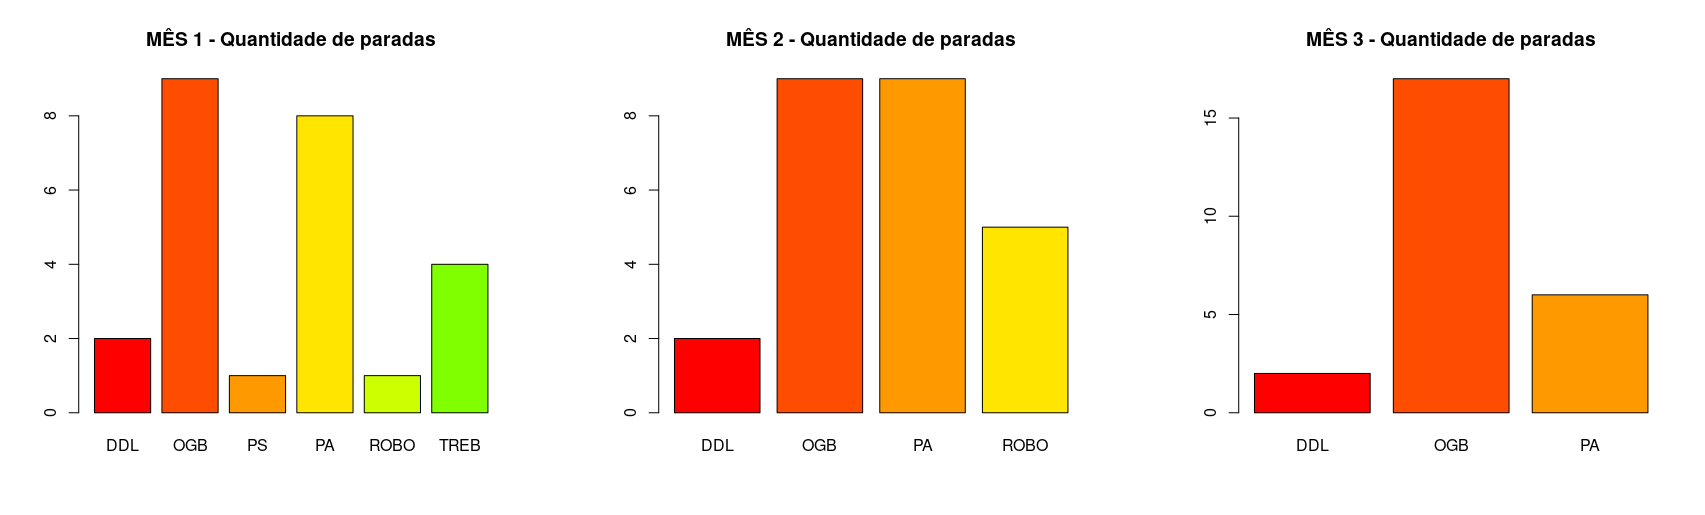
\includegraphics[ width=1\textwidth]{qtdparadas.png}
%         %\caption{.}
%     \end{figure}


%     \note[item]{Notes can help you to remember important information. Turn on the notes option.}
% \end{frame}
%-

%*----------- SLIDE -------------------------------------------------------------
% \begin{frame}[c]{Tempo de parada}
%     \centering
%     \begin{figure}
%         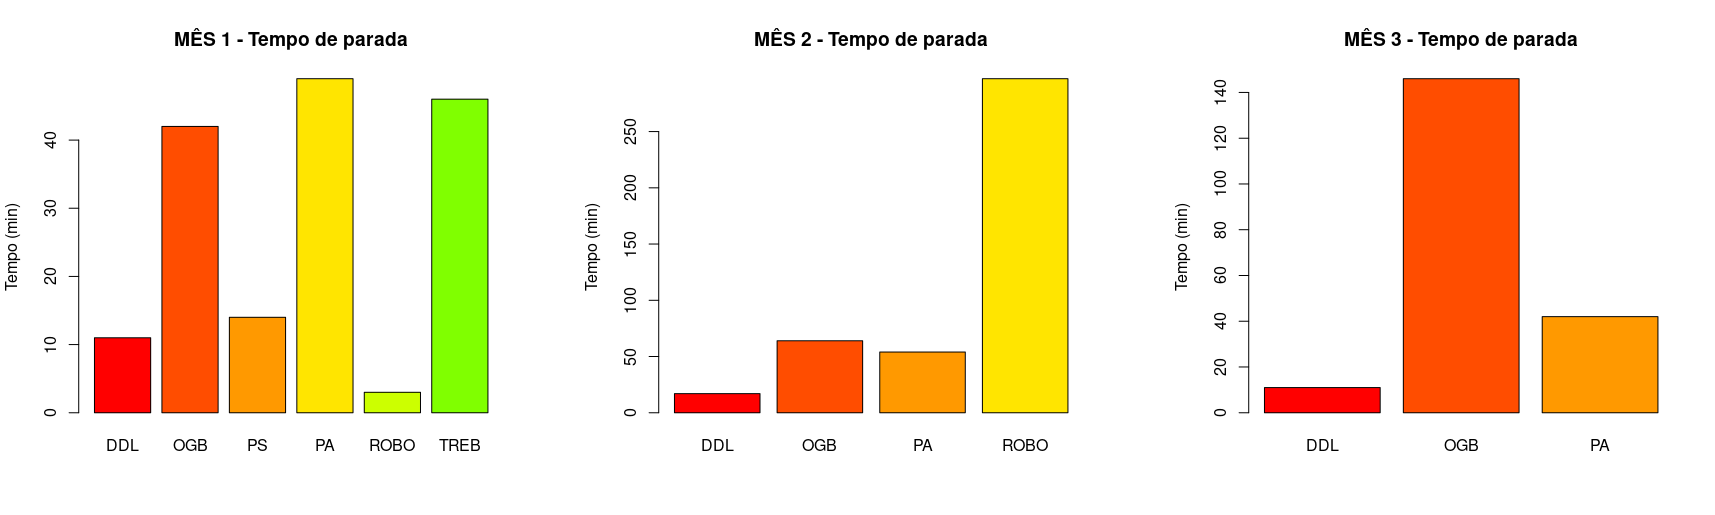
\includegraphics[ width=1\textwidth]{tempoparada.png}
%     \end{figure}

%*----------- notes
%     \note[item]{Notes can help you to remember important information. Turn on the notes option.}
% \end{frame}
%-

%*----------- SLIDE -------------------------------------------------------------
\begin{frame}[c]{Quantidade de paradas}
    \centering
    \begin{figure}
        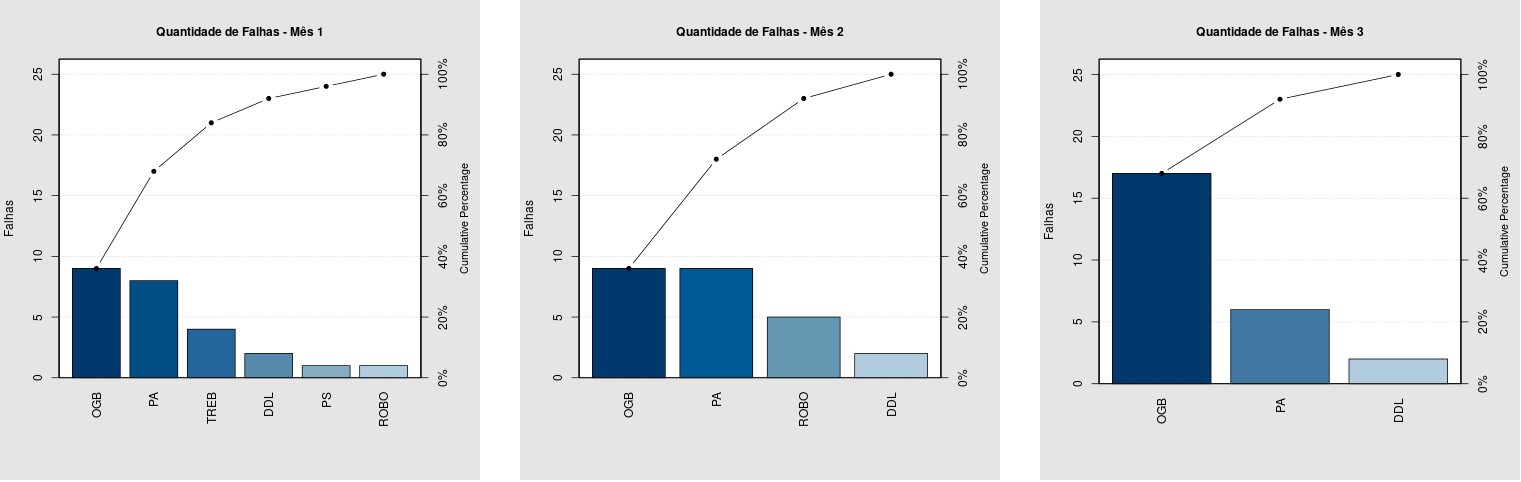
\includegraphics[ width=1\textwidth]{qtd-paradas.png}
        %\caption{.}
    \end{figure}

%*----------- notes
    \note[item]{Notes can help you to remember important information. Turn on the notes option.}
\end{frame}
%-

%*----------- SLIDE -------------------------------------------------------------
\begin{frame}[c]{Tempo de parada}
    \centering
    \begin{figure}
        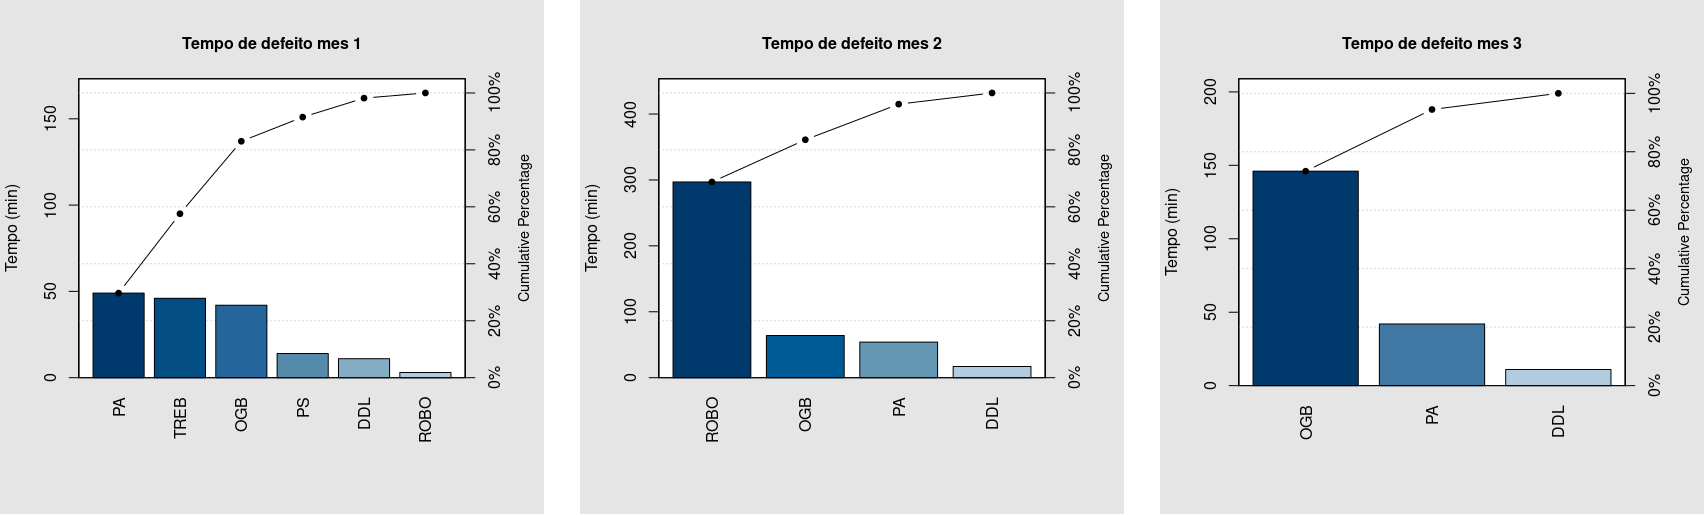
\includegraphics[ width=1\textwidth]{pareto.png}
        %\caption{.}
    \end{figure}

%*----------- notes
    \note[item]{Notes can help you to remember important information. Turn on the notes option.}
\end{frame}
%-
%*----------- SLIDE -------------------------------------------------------------
\begin{frame}[c]{Análise do problema}
    \centering
    \begin{figure}
        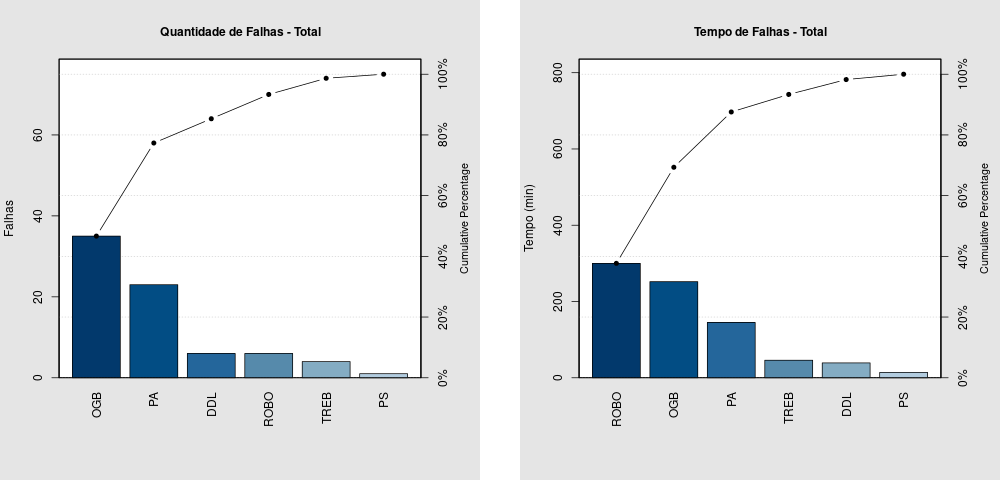
\includegraphics[ width=0.8\textwidth]{tempo-total.png}
        %\caption{.}
    \end{figure}

%*----------- notes
    \note[item]{Notes can help you to remember important information. Turn on the notes option.}
\end{frame}
%-

%*----------- SLIDE -------------------------------------------------------------
\begin{frame}[c]{Análise do problema}
    \begin{table}[ht!]
        \centering
            \caption{Análise considerando a planta}
            \begin{tabular}{|l|c|c|c|} \hline
                \textbf{Dados}&\textbf{Mês 1}&\textbf{Mês 2}&\textbf{Mês 3}\\ \hline
                Quantidade de falhas & 25  & 25  & 25\\ \hline
                Tempo parada &  165 min  & 432 min  &  199 min\\ \hline
                Tempo operacional & 9600 min & 9600 min & 9600 min \\ \hline
                Tempo disponível & 9435 min  & 9168 min  & 9401 min\\ \hline
                MTBF  & 6.29 h  & 6.112 h &  6.267 h\\ \hline
                MTTR  & 6.6 min  & 17.28 min &  7.96 min\\ \hline
            \end{tabular}
        \end{table}
%*----------- notes
    \note[item]{Notes can help you to remember important information. Turn on the notes option.}
\end{frame} 
%-

%*----------- SLIDE -------------------------------------------------------------
\begin{frame}[c]{Análise do problema}
    \centering
        \begin{table}[ht!]
            \centering
                \caption{Análise considerando os equipamentos}
                \begin{tabular}{|l|c|c|c|} \hline
                    \textbf{Dados}&\textbf{\Circled[outer color=mracula7, inner ysep=10pt]{Open Gate - B}}&\textbf{Pinça Automática}&\textbf{Robô}\\ \hline
                    Quantidade de falhas & 35  & 23  & 6\\ \hline
                    Tempo parada &  252 min  & 145 min  &  300 min\\ \hline
                    MTTR  & 7.2 min  & 6.30 min &  50 min\\ \hline
                \end{tabular}
            \end{table}

%*----------- notes
    \note[item]{Notes can help you to remember important information. Turn on the notes option.}
\end{frame}
%-